\chapter{Prototipo 4: Desarrollo de un sistema híbrido de recomendación de platillos}
  \section{Análisis}
    \subsection{Objetivo}
      Desarrollar un sistema híbrido para la recomendación de platillos que conlleve la demostración de la funcionalidad proporcionada por el API en un caso de estudio particular.

    \subsection{Características}
    \begin{itemize}
      \item El sistema permitirá realizar recomendaciones de platillos de acuerdo a sus características de los mismos (basadas en contenido).
      \item El sistema permitirá realizar recomendaciones de platillos con base en la interacción de los usuarios finales a través de ratings o evaluaciones cuantitativas (por filtrado colaborativo).
      \item El sistema permitirá el registro de usuarios finales, así como su autenticación para el uso de las funcionalidades del sistema.
      \item El sistema permitirá la visualización de los platillos a los usuarios no registrados.
      \item El sistema permitirá la recomendación para los usuarios no registrados a través del manejo de cookies en el navegdor y su interacción con los platillos.
    \end{itemize}

    \subsection{Restricciones}
    \begin{itemize}
      \item El sistema se verá limitado a las características y cantidad de platillos registrados para realizar las recomendaciones.
      \item El sistema no permitirá el registro de platillos a usuarios no registrados.
    \end{itemize}

    % Insertar historias de usuario aqui

  \section{Diseño}

    Para desarrollar las características mencionadas previamente, se debe tomar en cuenta el modelo de datos propio del caso de estudio que podemos observar en la figura ~\ref{fig:model_cs}

    \begin{landscape}
      \begin{figure}[h!]
        \centering
        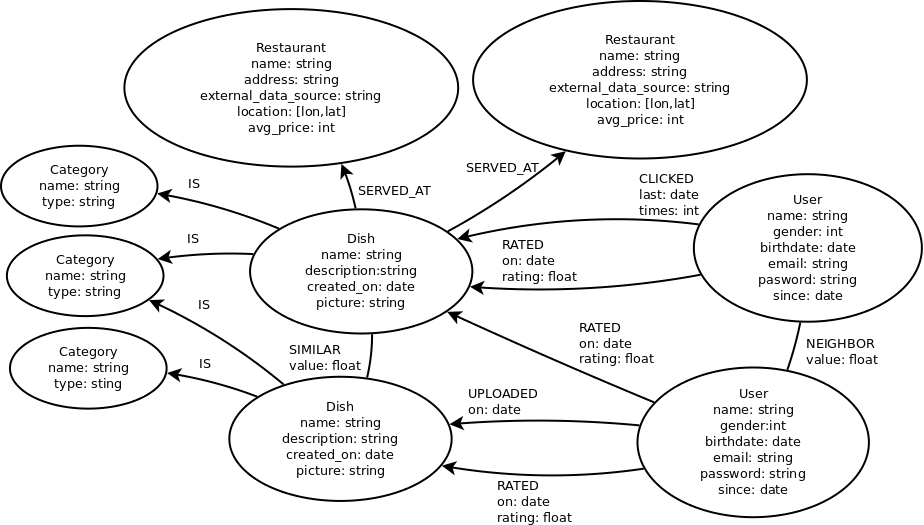
\includegraphics[width=25cm]{./images/sc_data_model}
        \caption{Modelo de datos del caso de estudio}
        \label{fig:model_cs}
      \end{figure}
    \end{landscape}

    % explique diseño de servicios aqui.
  
  \section{Resultados}
    Utilizando el comportamiento de la API como parte de la funcionalidad del sistema, integrado con las clases de dominio y los servicios diseñados previamente obtenemos la estructura mostrada en el diagrama de clases de la figura~\ref{fig:monster_classes}. 

    \begin{landscape}
      \begin{figure}[h!]
        \centering
        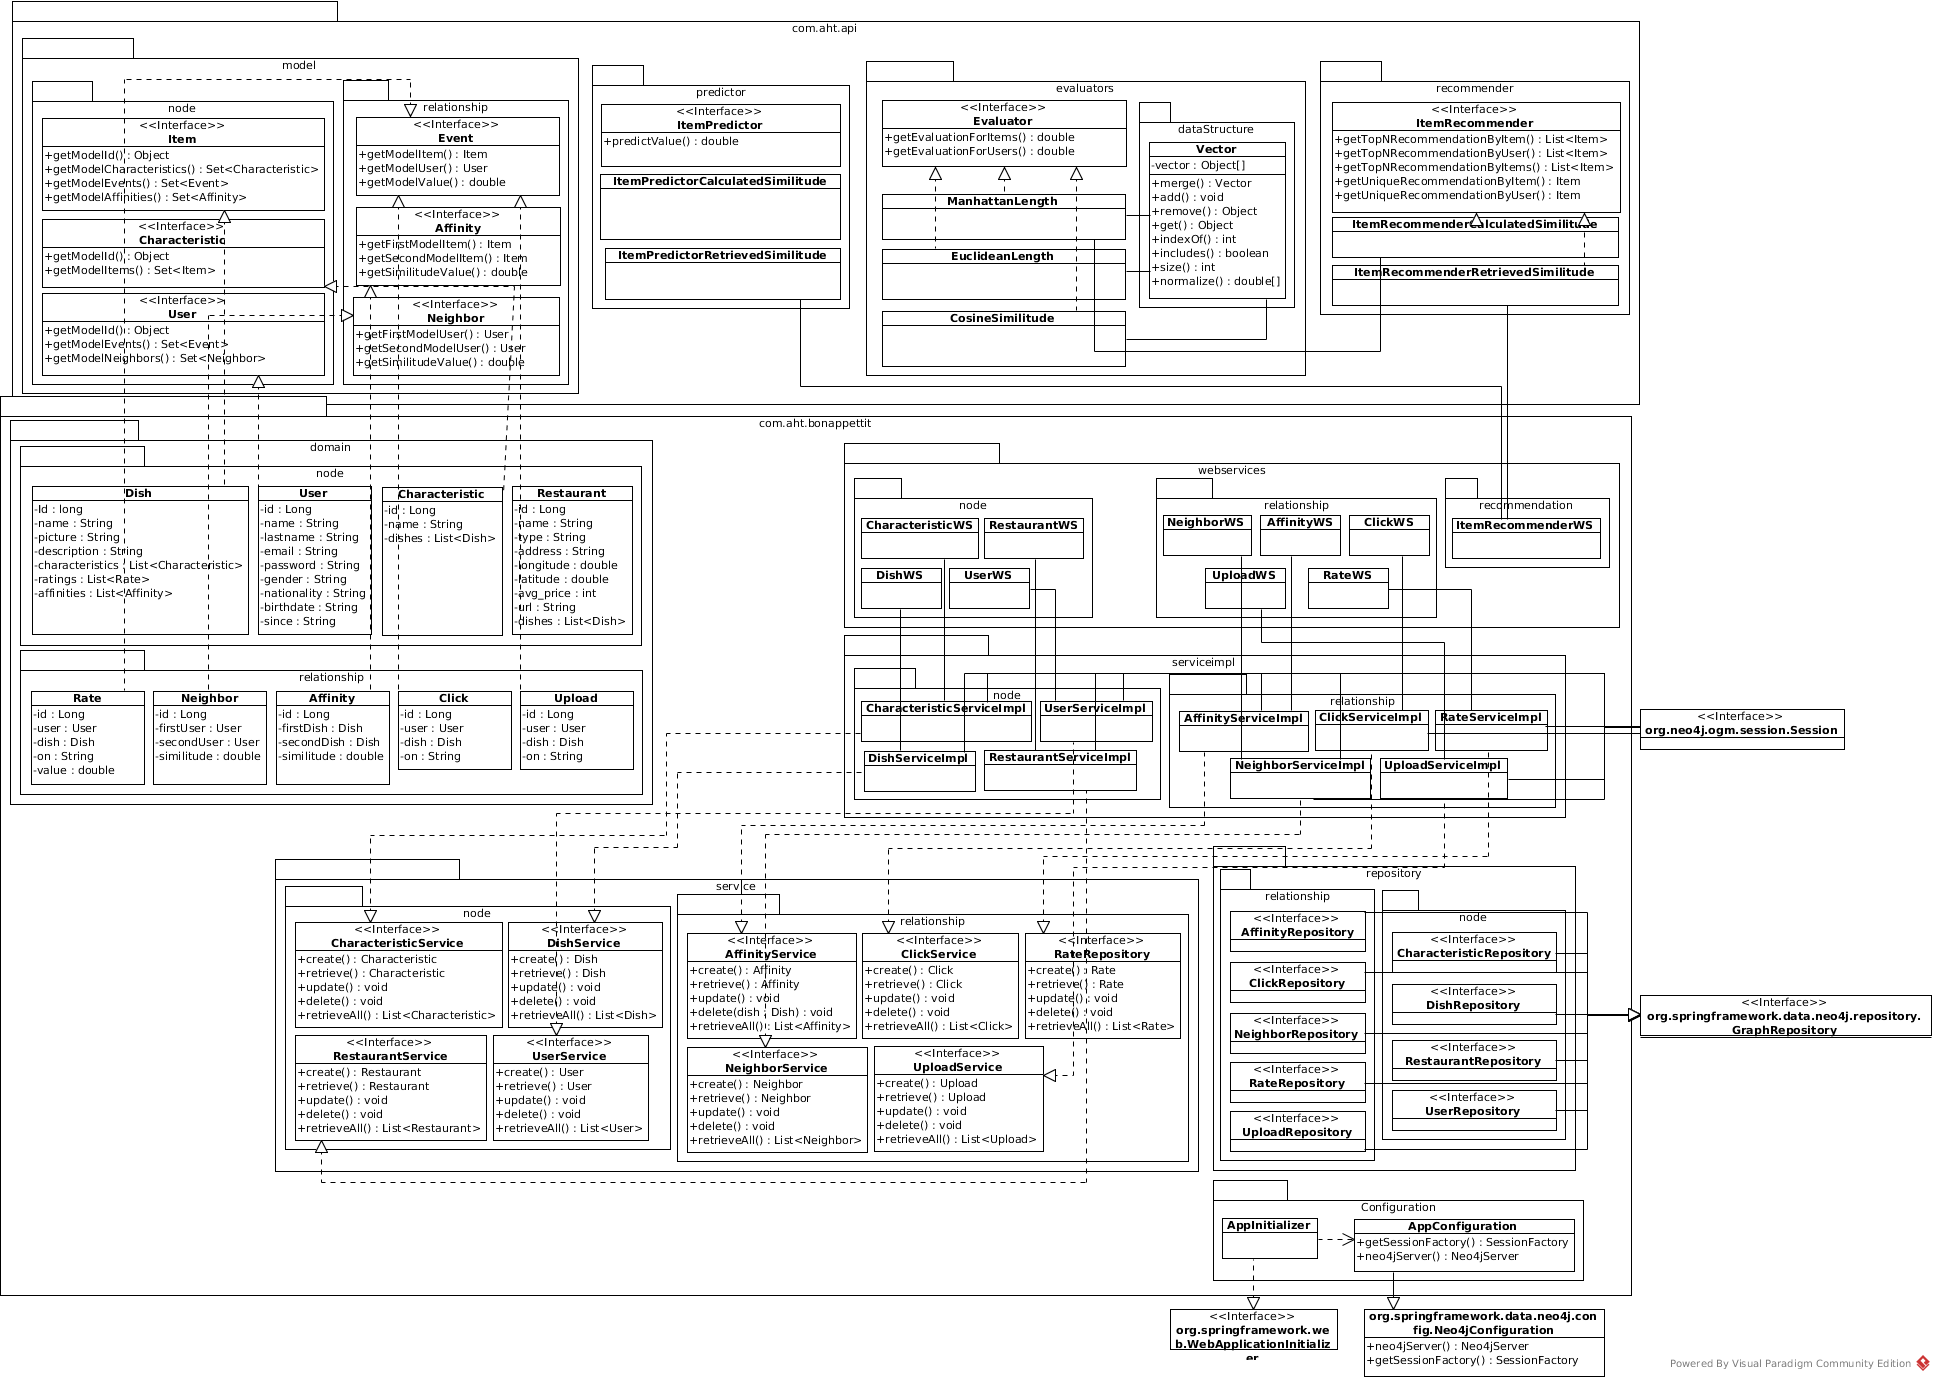
\includegraphics[width=25cm]{./images/monster_class}
        \caption{Diagrama de clases del prototipo 4}
        \label{fig:monster_classes}
      \end{figure}
    \end{landscape}

    Así finalmente podemos desarrollar el sistema, consumiendo los servicios web proporcionados por el back-end del sistema en una aplicación de angular, que a través de servicios y controladores que siguen el patrón MVC, permiten mostrar los datos en una interfaz gráfica al usuario final, como la mostrada en la figura~\ref{fig:final_bonappettit}


      \begin{figure}[h!]
        \centering
        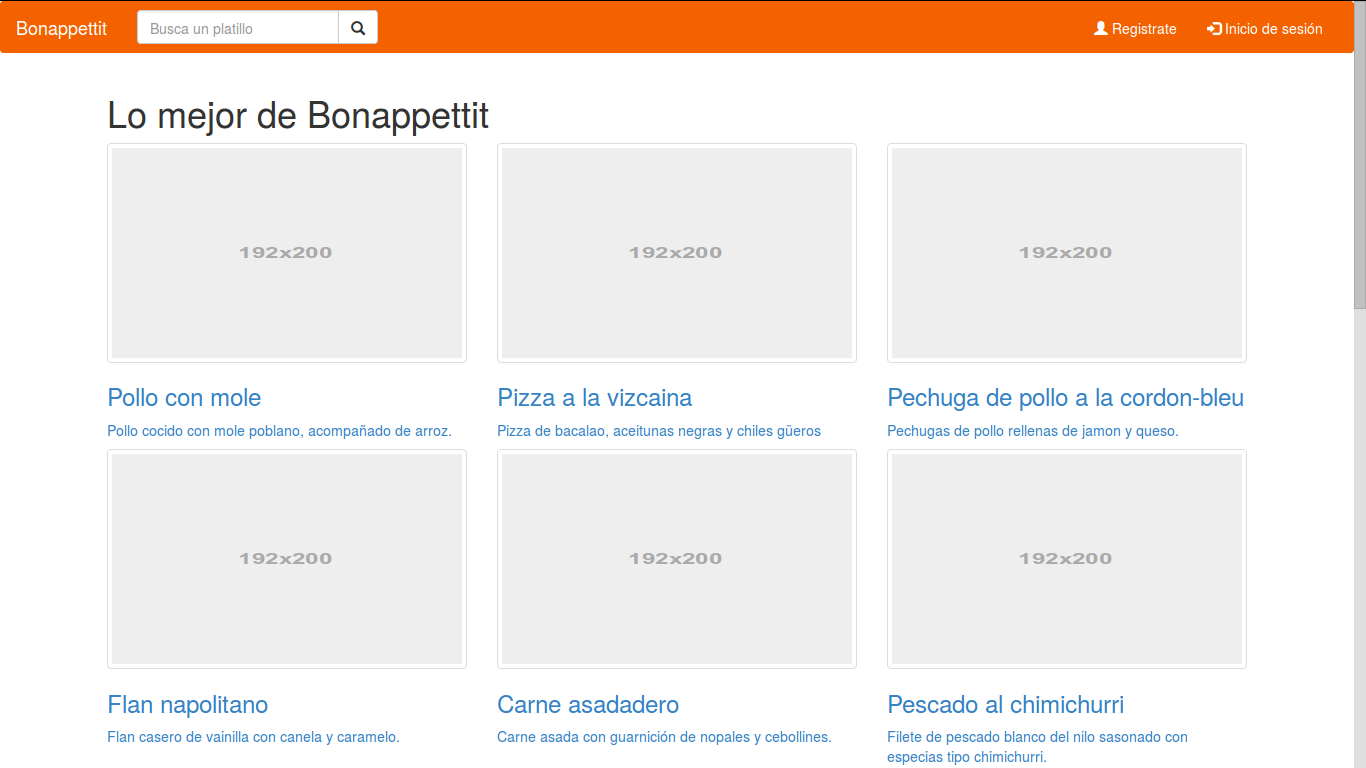
\includegraphics[width=16cm]{./images/p4_bonappettit}
        \caption{Interfaz gráfica del sistema}
        \label{fig:final_bonappettit}
      \end{figure}

